\begin{table*}[htbp]
  \centering
  \caption{AUC values of the 9 considered detectors on 12 datasets. \\ The best performance is shown in \textbf{bold} and the second best is \underline{underlined}.}
  \begin{tabular}{lccccccccc}
    \toprule
    Data$\setminus$Model & RXD~\cite{RXD} & CRD~\cite{CRD} & GAED~\cite{GAED} & MSNet~\cite{MSNet} & PDBSNet~\cite{PDBSNet} & PTA~\cite{PTA} & AutoAD~\cite{AutoAD} & RGAE~\cite{RGAE} & SuperAD (Ours) \bigstrut \\
    \hline
    Texas Coast & 0.9906 & 0.9910 & 0.9779 & 0.9946 & \underline{0.9950} & 0.6992 & 0.9938 & 0.9709 & \textbf{0.9982} \bigstrut[t] \\
    San Diego & 0.9089 & 0.8608 & 0.9866 & \underline{0.9907} & 0.9820 & 0.9683 & 0.9849 & 0.6991 & \textbf{0.9929} \bigstrut[t] \\
    HYDICE Urban & 0.9933 & 0.9975 & 0.9845 & 0.9993 & 0.9996 & 0.8659 & \textbf{0.9998} & 0.7064 & \underline{0.9993} \bigstrut[t] \\
    Pavia & 0.9537 & 0.9167 & 0.9362 & 0.9889 & \underline{0.9892} & 0.9061 & 0.9818 & 0.9053 & \textbf{0.9911} \bigstrut[t] \\
    ABU-Airport-1 & 0.8380 & 0.8481 & 0.8747 & \textbf{0.9582} & 0.9279 & 0.6504 & 0.9179 & 0.7773 & \underline{0.9418} \bigstrut[t] \\
    ABU-Airport-2 & 0.9502 & 0.7902 & 0.9049 & 0.9445 & \underline{0.9834} & 0.9663 & 0.9915 & 0.6698 & \textbf{0.9965} \bigstrut[t] \\
    ABU-Beach-1 & 0.9531 & \textbf{0.9960} & 0.9184 & 0.9580 & 0.9610 & 0.9303 & 0.9787 & 0.9470 & \underline{0.9844} \bigstrut[t] \\
    ABU-Beach-2 & 0.9106 & 0.9248 & 0.5444 & 0.9129 & \underline{0.9518} & 0.0960 & 0.9374 & 0.9049 & \textbf{0.9627} \bigstrut[t] \\
    ABU-Urban-1 & 0.9926 & 0.9394 & 0.9993 & \underline{0.9994} & 0.9994 & 0.8161 & 0.9960 & 0.9993 & \textbf{0.9994} \bigstrut[t] \\
    ABU-Urban-2 & 0.9501 & 0.9420 & 0.9591 & 0.9767 & \underline{0.9864} & 0.5087 & 0.9772 & 0.8249 & \textbf{0.9943} \bigstrut[t] \\
    ABU-Urban-3 & 0.9878 & 0.9719 & 0.9938 & \underline{0.9966} & 0.9966 & 0.4826 & 0.9908 & 0.9965 & \textbf{0.9970} \bigstrut[t] \\
    ABU-Urban-4 & 0.9685 & 0.8986 & 0.8104 & 0.9700 & \underline{0.9724} & 0.5192 & 0.9573 & 0.9651 & \textbf{0.9864} \bigstrut[t] \\
    \midrule
    Average & 0.9498 & 0.9231 & 0.9075 & 0.9741 & \underline{0.9787} & 0.7007 & 0.9756 & 0.8639 & \textbf{0.9870} \bigstrut[t] \\
    \bottomrule
  \end{tabular}%
  \label{tab:cmp-all-models}%
\end{table*}


\begin{figure*}[htbp]
  \centering
  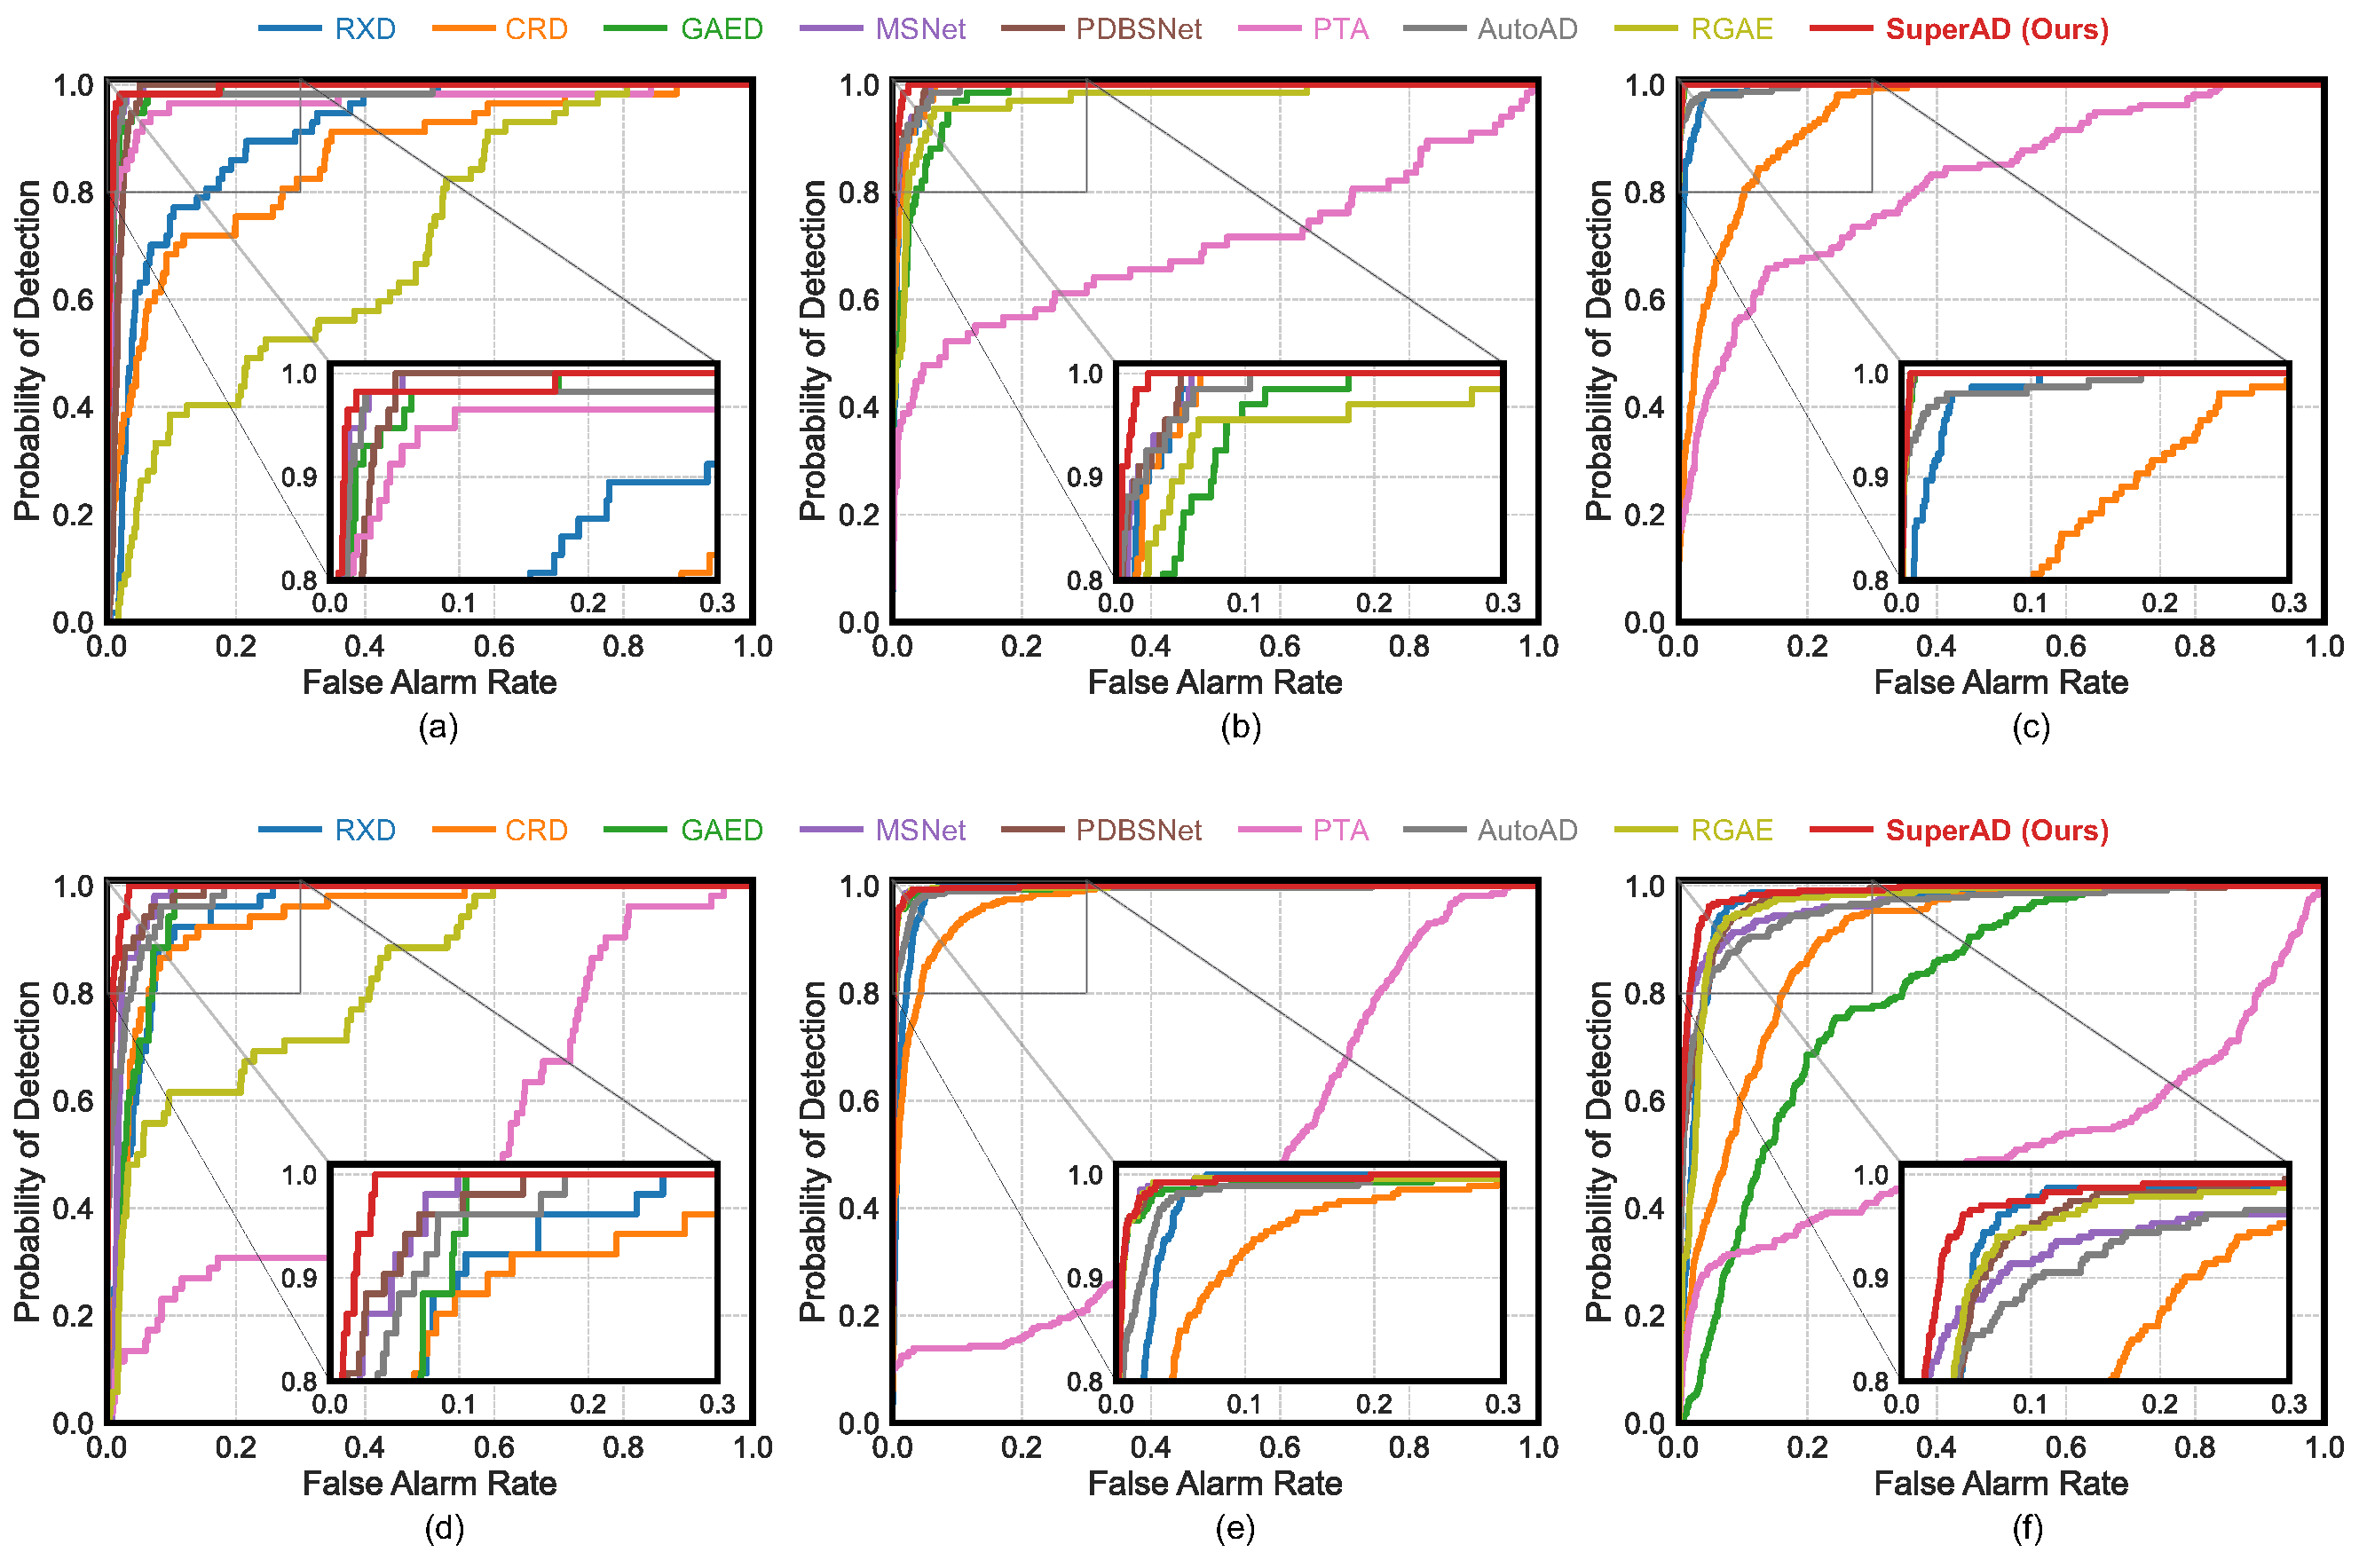
\includegraphics[width=1\linewidth]{Figures/PDF/roc_all.pdf}
  \caption{ROC curves of the 9 considered detectors on (a) San Diego, (b) Texas Coast, (c) ABU-Urban-1, (d) ABU-Urban-2, (e) ABU-Urban-3, and (f) ABU-Urban-4.}
  \label{fig:cmp-all-models-roc}
\end{figure*}

\begin{figure*}[htbp]
    \centering
    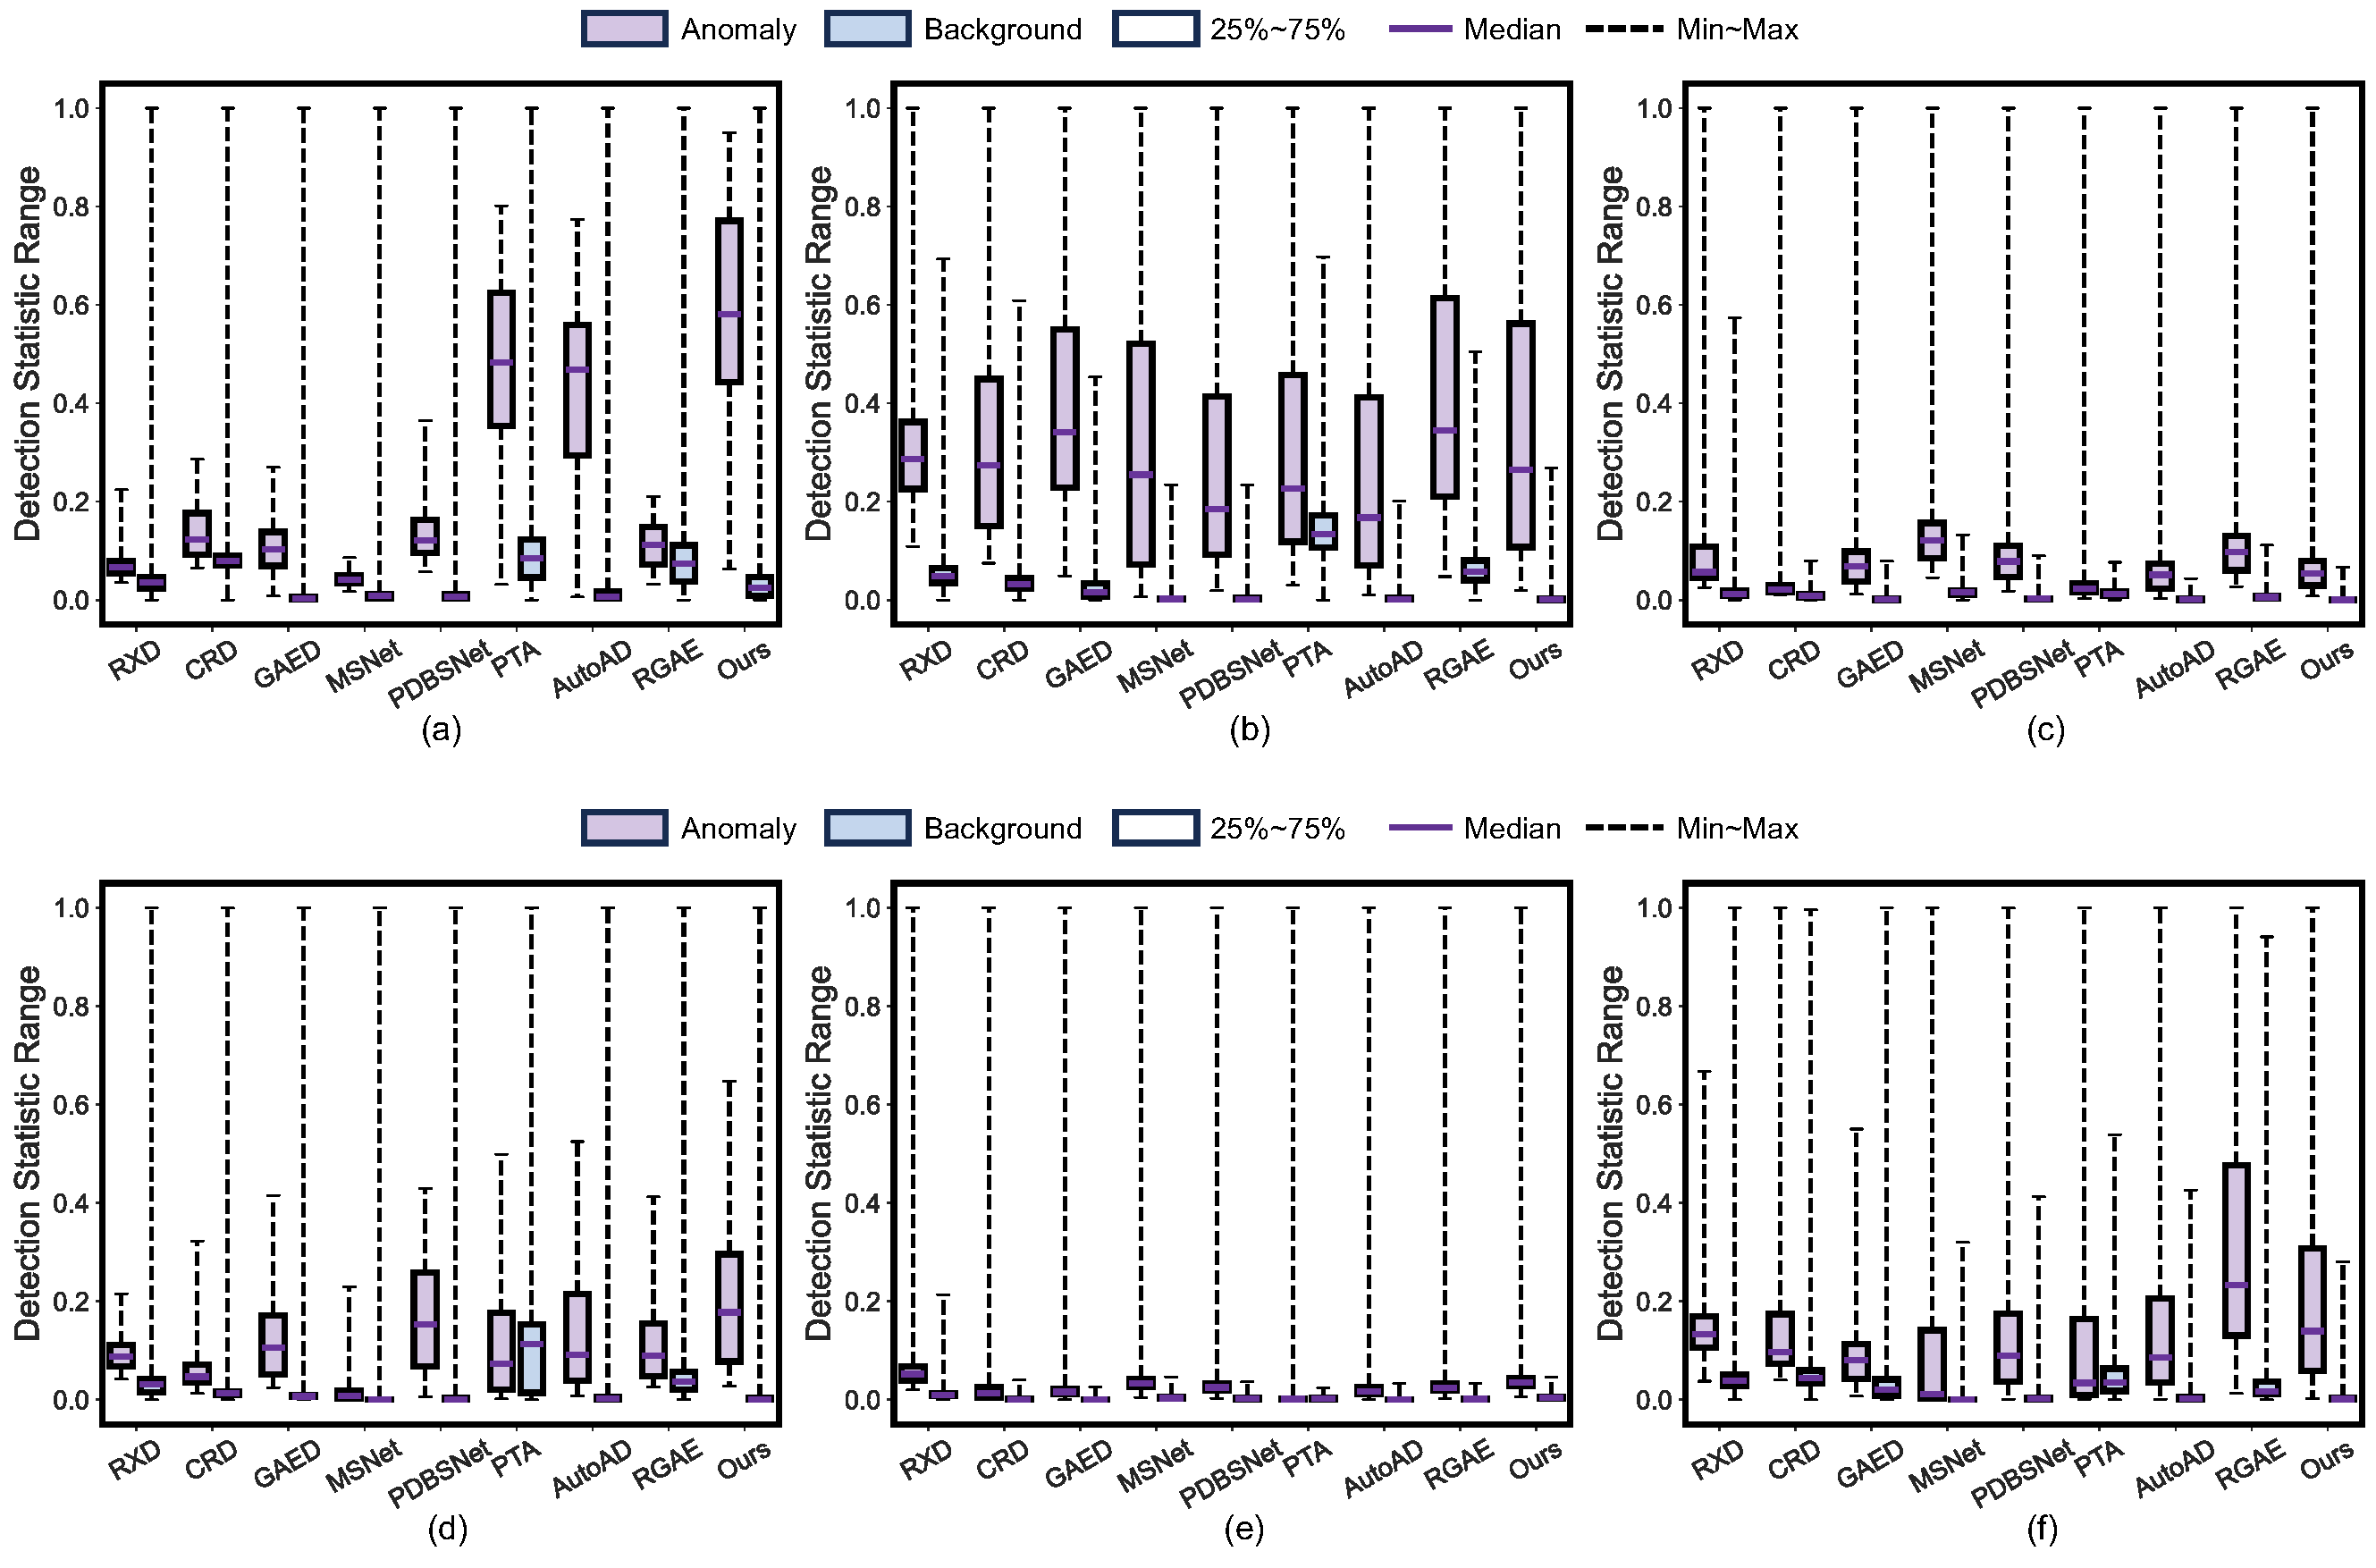
\includegraphics[width=1\linewidth]{Figures/PDF/box_all.pdf}
    \caption{Separability maps of the 9 considered detectors on (a) San Diego, (b) Texas Coast, (c) ABU-Urban-1, (d) ABU-Urban-2, (e) ABU-Urban-3, and (f) ABU-Urban-4.}
    \label{fig:cmp-all-models-box}
  \end{figure*}
  


% $\hat{\mathrm{\mathbf{M}}} \in \mathbb{R}^{h\times w}$, $ \mathrm{\mathbf{F}} \in \mathbb{R}^{h\times w}$ 

\begin{figure*}[htbp]
  \centering
  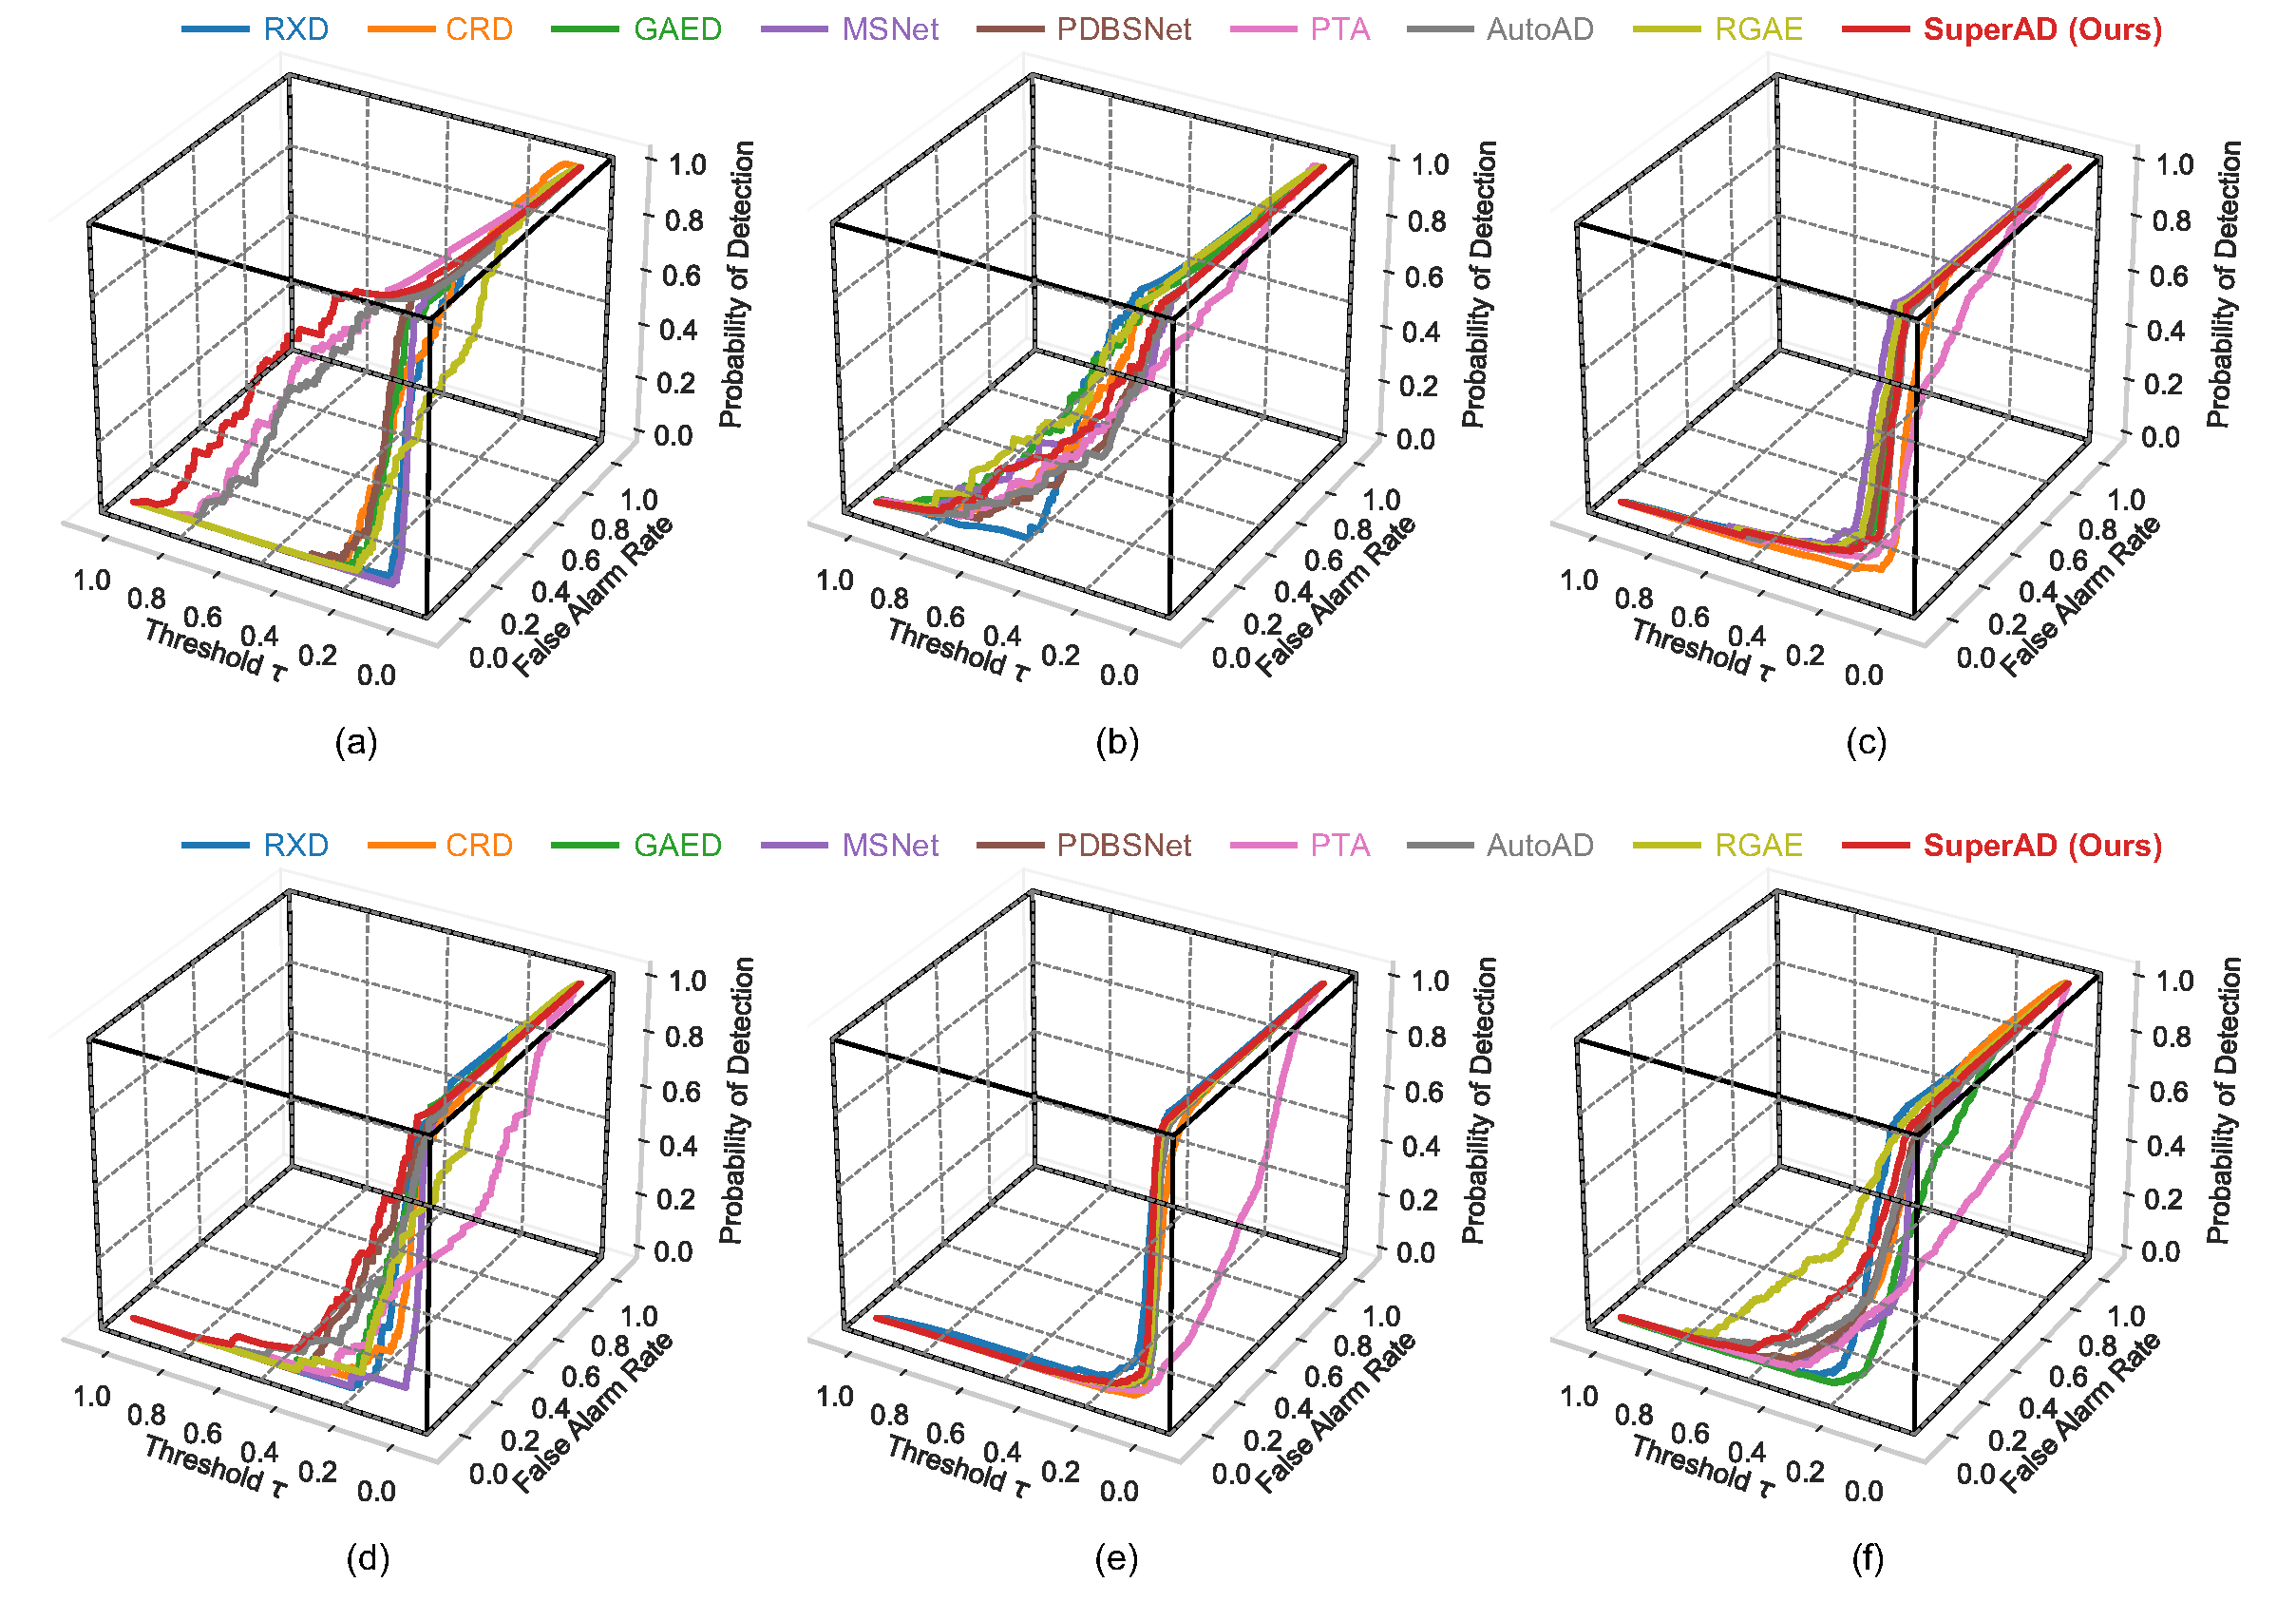
\includegraphics[width=1\linewidth]{Figures/PDF/3droc_all.pdf}
  \caption{3D-ROC curves of the 9 considered detectors on (a) San Diego, (b) Texas Coast, (c) ABU-Urban-1, (d) ABU-Urban-2, (e) ABU-Urban-3, and (f) ABU-Urban-4.}
  \label{fig:cmp-all-models-3droc}
\end{figure*}


\section{Experimental Results}\label{Experimentss}




\subsection{Experimental Settings}




We evaluate the performance of our methods using seven widely recognized hyperspectral datasets: Texas Coast, San Diego, HYDICE Urban, Pavia, ABU-Airport, ABU-Beach and ABU-Urban. Eight commonly-recognized models including tranditional RXD~\cite{RXD} and CRD~\cite{CRD}, and self-supervised methods with diverse architectures including GAED~\cite{GAED}, MSNet~\cite{MSNet}, PDBSNet~\cite{PDBSNet}, PTA ~\cite{PTA}, AutoAD ~\cite{AutoAD}, and RGAE~\cite{RGAE}, were compared with the proposed methods.
The network architecture was implemented using PyTorch. All experiments were conducted on an NVIDIA GeForce RTX 2080 Ti with 11 GB of memory. Access the source code: \url{https://github.com/yc-cui/Super-AD}.

\begin{figure*}[htbp]
  \centering
  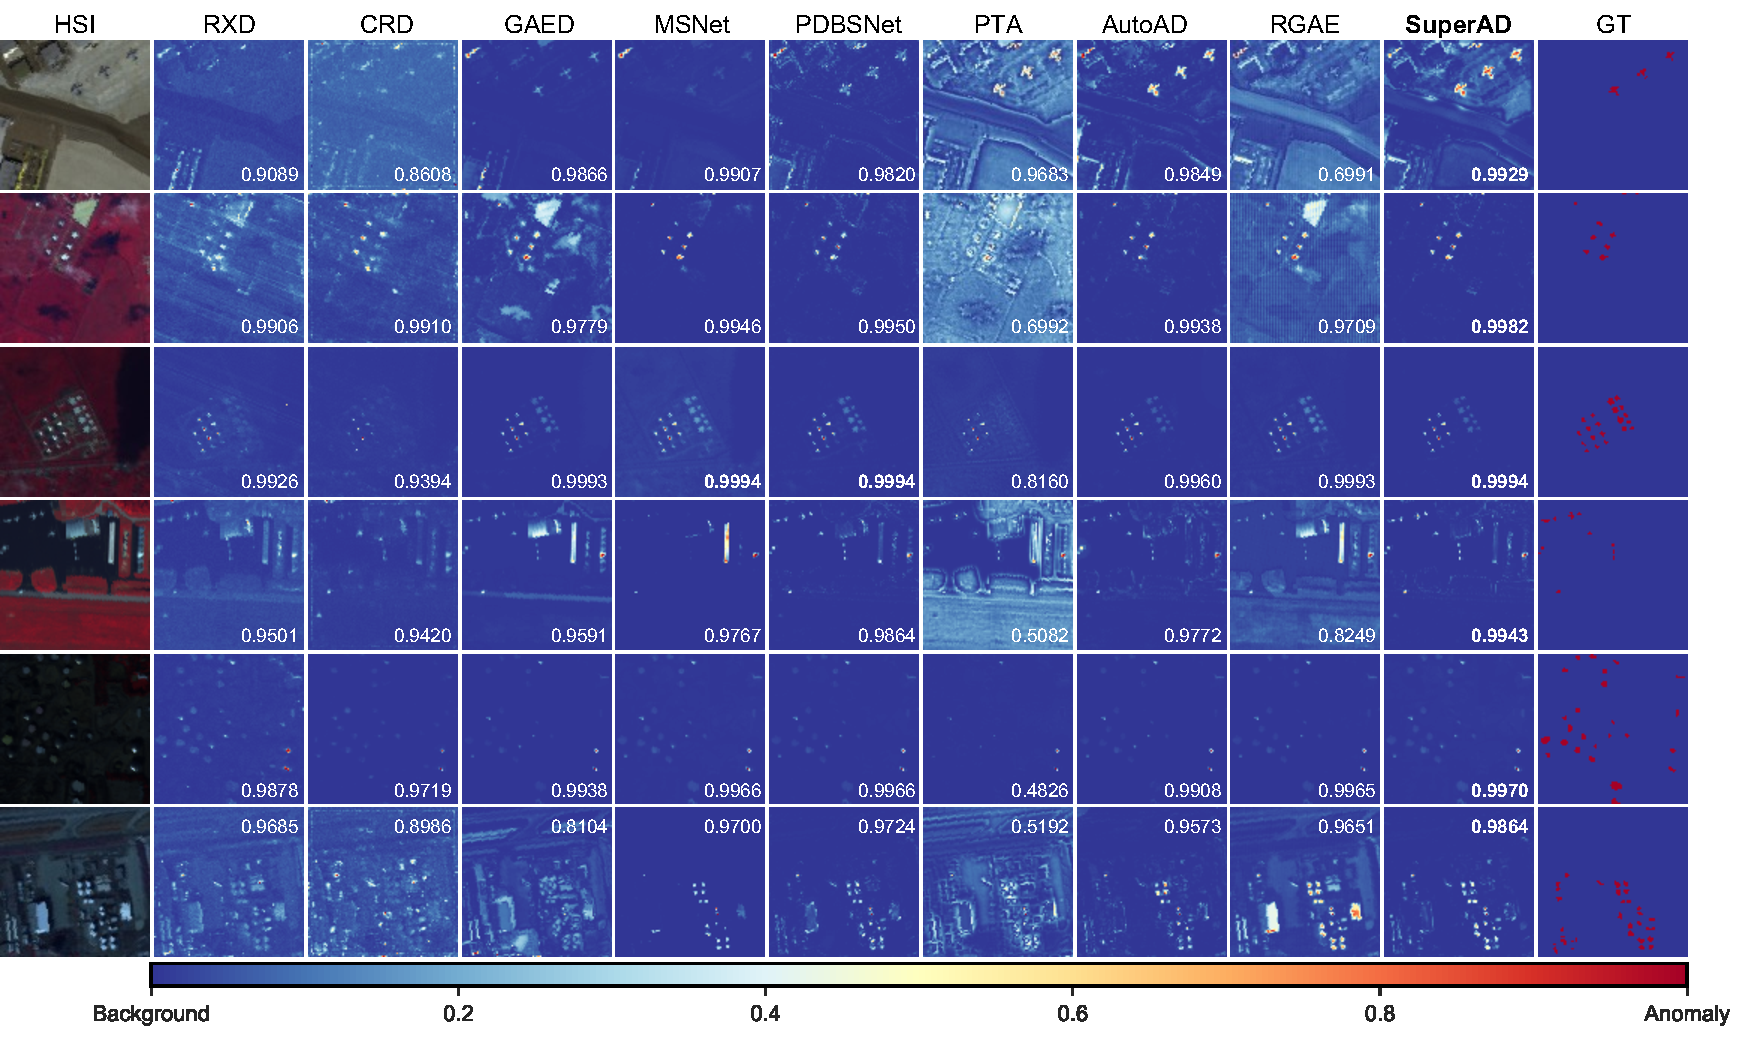
\includegraphics[width=1\linewidth]{Figures/PDF/cmp_all.pdf}
  \caption{Visualization of detection results of the 9 considered detectors on (from top to bottom) San Diego, Texas Coast, ABU-Urban-1, ABU-Urban-2, ABU-Urban-3, and ABU-Urban-4. }
  \label{fig:cmp-all-models}
\end{figure*}



\subsection{Detection Performance Comparison}



\subsubsection{Quantitative Comparison}
As shown in Table \ref{tab:cmp-all-models}, our model obtained leading results in terms of AUC across the majority of the datasets. The performance differences between the datasets can be attributed to their distinct spectral-spatial features. On the San Diego dataset ($0.9982$ AUC), the anomalies (three airplanes with structural information) contrast spectrally with the background, and our spectral perturbation strategy significantly reduces the background interference. Although the performance is slightly degraded on the HYDICE Urban dataset ($0.9993$ vs. $0.9998$), where the vehicles and roofs are considered anomalies with $21$ anomalous pixels constituting about $0.26$\% of the entire image, the adaptive-weighted loss function in AutoAD~\cite{AutoAD} shows a localized advantage. But overall performance remains competitive. The comparative analysis of the receiver operating characteristic curve (ROC) presented in Fig.~\ref{fig:cmp-all-models-roc} and the separability maps shown in Fig.~\ref{fig:cmp-all-models-box} across all seven datasets further validates the superior ability of the proposed model to distinguish anomalies from background compared to other models. This consistent improvement highlights the effectiveness of our spectral perturbation strategy in enhancing feature discrimination.            

To further assess the effectiveness of the model, Fig.~\ref{fig:cmp-all-models-3droc} illustrates the comparative results of the three-dimensional ROC (3DROC) curves~\cite{chang2020effective,song20203}. 3DROC extends the evaluation dimensions of the traditional ROC by introducing a detection threshold $\tau$, whose key metric, the signal-to-noise ratio (SNPR), is calculated as:

\begin{equation}
\text{SNPR} = 10 \cdot \log_{10}\left(\frac{A_{\text{PD-}\tau}}{A_{\text{PF-}\tau}}\right)
\end{equation}

where $A_{\text{PD-}\tau}$ and $A_{\text{PF-}\tau}$ denote the area under the curve of the detection rate-threshold curve and false alarm rate-threshold curve, respectively. The experimental results demonstrate three key advantages of our method: First, in the PD-PF plane, our curve shows the closest proximity to the upper-right boundary with the largest $A_{\text{PD-PF}}$ area, indicating optimal detection rate-false-alarm rate trade-off across all threshold values. Second, the PD-$\tau$ projection reveals significantly larger $A_{\text{PD-}\tau}$ area compared to baseline methods, confirming superior target capture capability even under strict threshold constraints. Third, while our $A_{\text{PF-}\tau}$ area is not the absolute minimum, the maximized signal-to-noise ratio enables exceptional robustness in anomaly discrimination within complex interference environments. This analysis shows that the proposed framework effectively suppresses the false alarm accumulation effect while maintaining high detection sensitivity through the synergistic action of spectral perturbation and adaptive regularization, a feature that is difficult to achieve in conventional methods.



% Table generated by Excel2LaTeX from sheet 'Sheet5'
\begin{table}[htbp]
  \centering
  \caption{Comparison of model parameters, computational complexity, and training time. \textbf{Bold} indicates the best performance. $^\dag$ indicates MATLAB code.}
  \begin{tabular}{lccc}
    \toprule
    Model                   & \#Params (M) & MACs (G) & Avg. Time \bigstrut \\
    \hline
    RXD~\cite{RXD}$^\dag$   & -            & -        & 01m 26s \bigstrut[t] \\
    CRD~\cite{CRD}$^\dag$   & -            & -        & 01m 31s \bigstrut[t] \\
    GAED~\cite{GAED}$^\dag$ & -            & -        & 01m 33s \bigstrut[t] \\
    MSNet~\cite{MSNet}      & 0.553        & 5.511    & 05m 49s \bigstrut[t] \\
    PDBSNet~\cite{PDBSNet}  & 0.687        & 5.459    & 14m 09s \bigstrut[t] \\
    PTA~\cite{PTA}$^\dag$   & -            & -        & \textbf{00m 53s} \bigstrut[t]    \\
    AutoAD~\cite{AutoAD}    & 3.249        & 5.979    & 06m 04s \bigstrut[t]  \\
    RGAE~\cite{RGAE}$^\dag$ & -            & -        & 02m 01s \bigstrut[t]  \\
    SuperAD (Ours)          & \textbf{0.241}        & \textbf{2.220}    & 05m 50s \bigstrut[t] \\
    \bottomrule
  \end{tabular}%
  \label{tab:cmp-efficiency}%
\end{table}%


\subsubsection{Visual Comparison}
Fig.~\ref{fig:cmp-all-models} illustrates the anomaly detection maps for the San Diego, Texas Coast, and ABU-Urban datasets. Among all the evaluated models, only MSNet~\cite{MSNet} and AutoAD~\cite{AutoAD} demonstrate competitive performance to our approach. While MSNet~\cite{MSNet} yields impressive results on the Texas Coast dataset, it struggles to identify anomalous pixels within the San Diego dataset. This may be due to the fact that the network is not designed for use in urban zones with complex background information. For AutoAD~\cite{AutoAD}, although it also exhibited strong performance, our model assigns higher probabilities to anomalous points compared to AutoAD~\cite{AutoAD}. This clearly indicates that the proposed model effectively differentiates anomalies from the background, highlighting the efficacy of our method. In practice, it is possible to consistently assign higher probabilities to true anomalies while minimizing false positives. The advanced of our model on different datasets demonstrates that the approach we employ (perturbation, reconstruction, and regularization) is suitable and robust for handling the complexity and variability present in different hyperspectral imaging scenarios. This consistent performance across datasets enhances the robustness and reliability of our approach in hyperspectral anomaly detection.



\subsubsection{Comparison of Model Efficiency}
The model complexity presented in Table~\ref{tab:cmp-efficiency} demonstrates the advantages of our proposed model according to the number of parameters and computational complexity. With only $0.241$ million parameters, our architecture achieves a significant reduction in model complexity compared to existing approaches such as AutoAD~\cite{AutoAD}. The computational complexity, measured in multiply-accumulate operations (MACs), further underscores the efficiency of our approach. The MACs was calculated for an input tensor of size $(1, 204, 100, 100)$. Our model requires less than half the computational resources of comparable methods. The training time reveals that our model maintains competitive efficiency, achieving performance comparable to MSNet~\cite{MSNet} while being significantly faster than PDBSNet~\cite{PDBSNet}.





\subsection{Ablation Study and Parameter Analysis}


\begin{table}[t]
  \centering
  \caption{Ablation of perturbation operation SPP.}
  \begin{tabular}{rccccc}
    \toprule
            & Coast           & San Diego       & HYDICE Urban          & Pavia           & Average \bigstrut[t]      \\
    \midrule
    w/o SPP & 0.9938          & 0.9905          & 0.9960          & 0.9847          & 0.9913 \bigstrut          \\
    w/ SPP  & \textbf{0.9982} & \textbf{0.9929} & \textbf{0.9993} & \textbf{0.9911} & \textbf{0.9954} \bigstrut \\
    \bottomrule
  \end{tabular}%
  \label{tab:abl-SPP}%
\end{table}%


\subsubsection{Perturbation Operation SPP}\label{sec:spp}
An ablation study was conducted to evaluate the contribution of the superpixel pooling and uppooling mechanism, as shown in Table \ref{tab:abl-SPP}. The results clearly demonstrate the significant impact of SPP on the model's performance, with a noticeable increase in AUC scores when SPP is incorporated. This indicates that SPP plays a crucial role in mitigating the IMP by encapsulating anomalous pixels within background-dominated blocks, thereby preventing their influence on the reconstruction process.





\begin{figure}[htbp]
  \centering
  {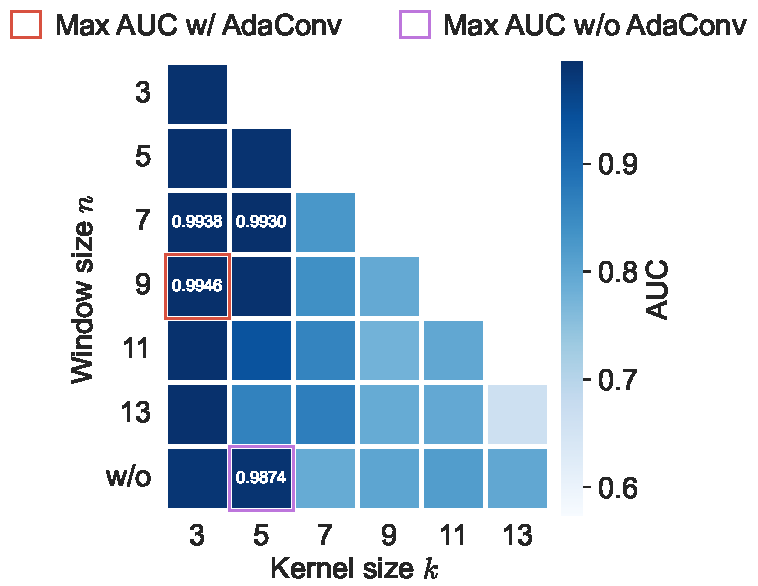
\includegraphics[width=0.6\linewidth]{abl_nk_2.pdf}}
  \caption{Ablation studies and parameter analysis conducted on San Diego dataset for AdaConv.}
  \label{fig:abl-nk}
\end{figure}


\subsubsection{Reconstruction Function AdaConv}
Fig.~\ref{fig:abl-nk} present the results of ablation studies and parameter analysis on the reconstruction function AdaConv. Optimal performance is achieved with a window size of $n=9$ and a kernel size of $k=3$, yielding an AUC of $0.9946$. We noticed AdaConv exhibits sensitivity to large kernels, such as \{7, 9, 11, 13\}, possibly due to the incorporation of irrelevant information by distant pixels, which diminishes the local correlation with the center pixel. As shown in the last row of Fig.~\ref{fig:abl-nk}, without AdaConv, the optimal AUC is $0.9874$. This indicates that AdaConv effectively targets non-anomalous pixels, enhancing the model's ability to reconstruct the background while disregarding anomalies, thereby preventing IMP and achieving superior results.




\begin{figure}[htbp]
  \centering
  {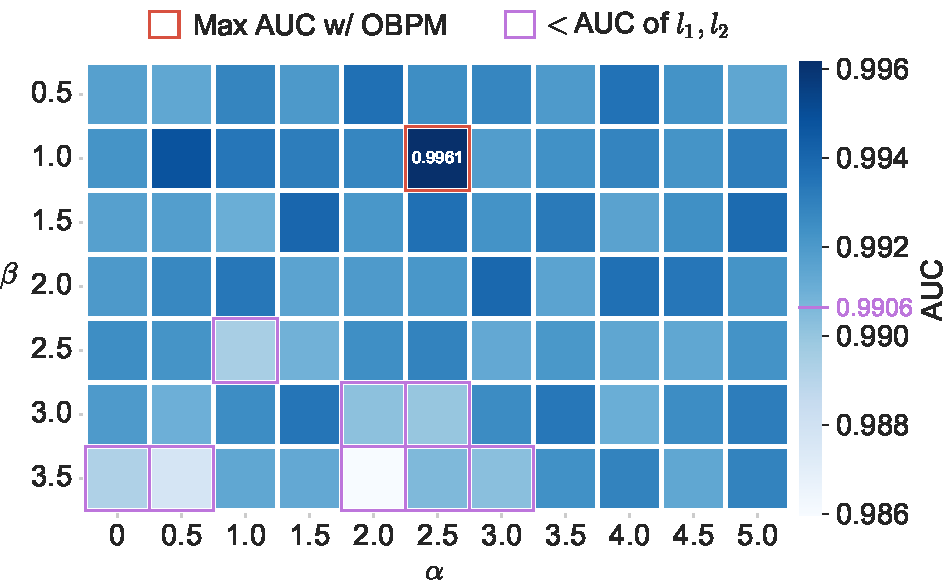
\includegraphics[width=0.8\linewidth]{abl_ab_2.pdf}}
  \caption{Ablation studies and parameter analysis conducted on San Diego dataset for OBPM.}
  \label{fig:abl-ab}
\end{figure}


\begin{figure*}[htbp]
  \centering
  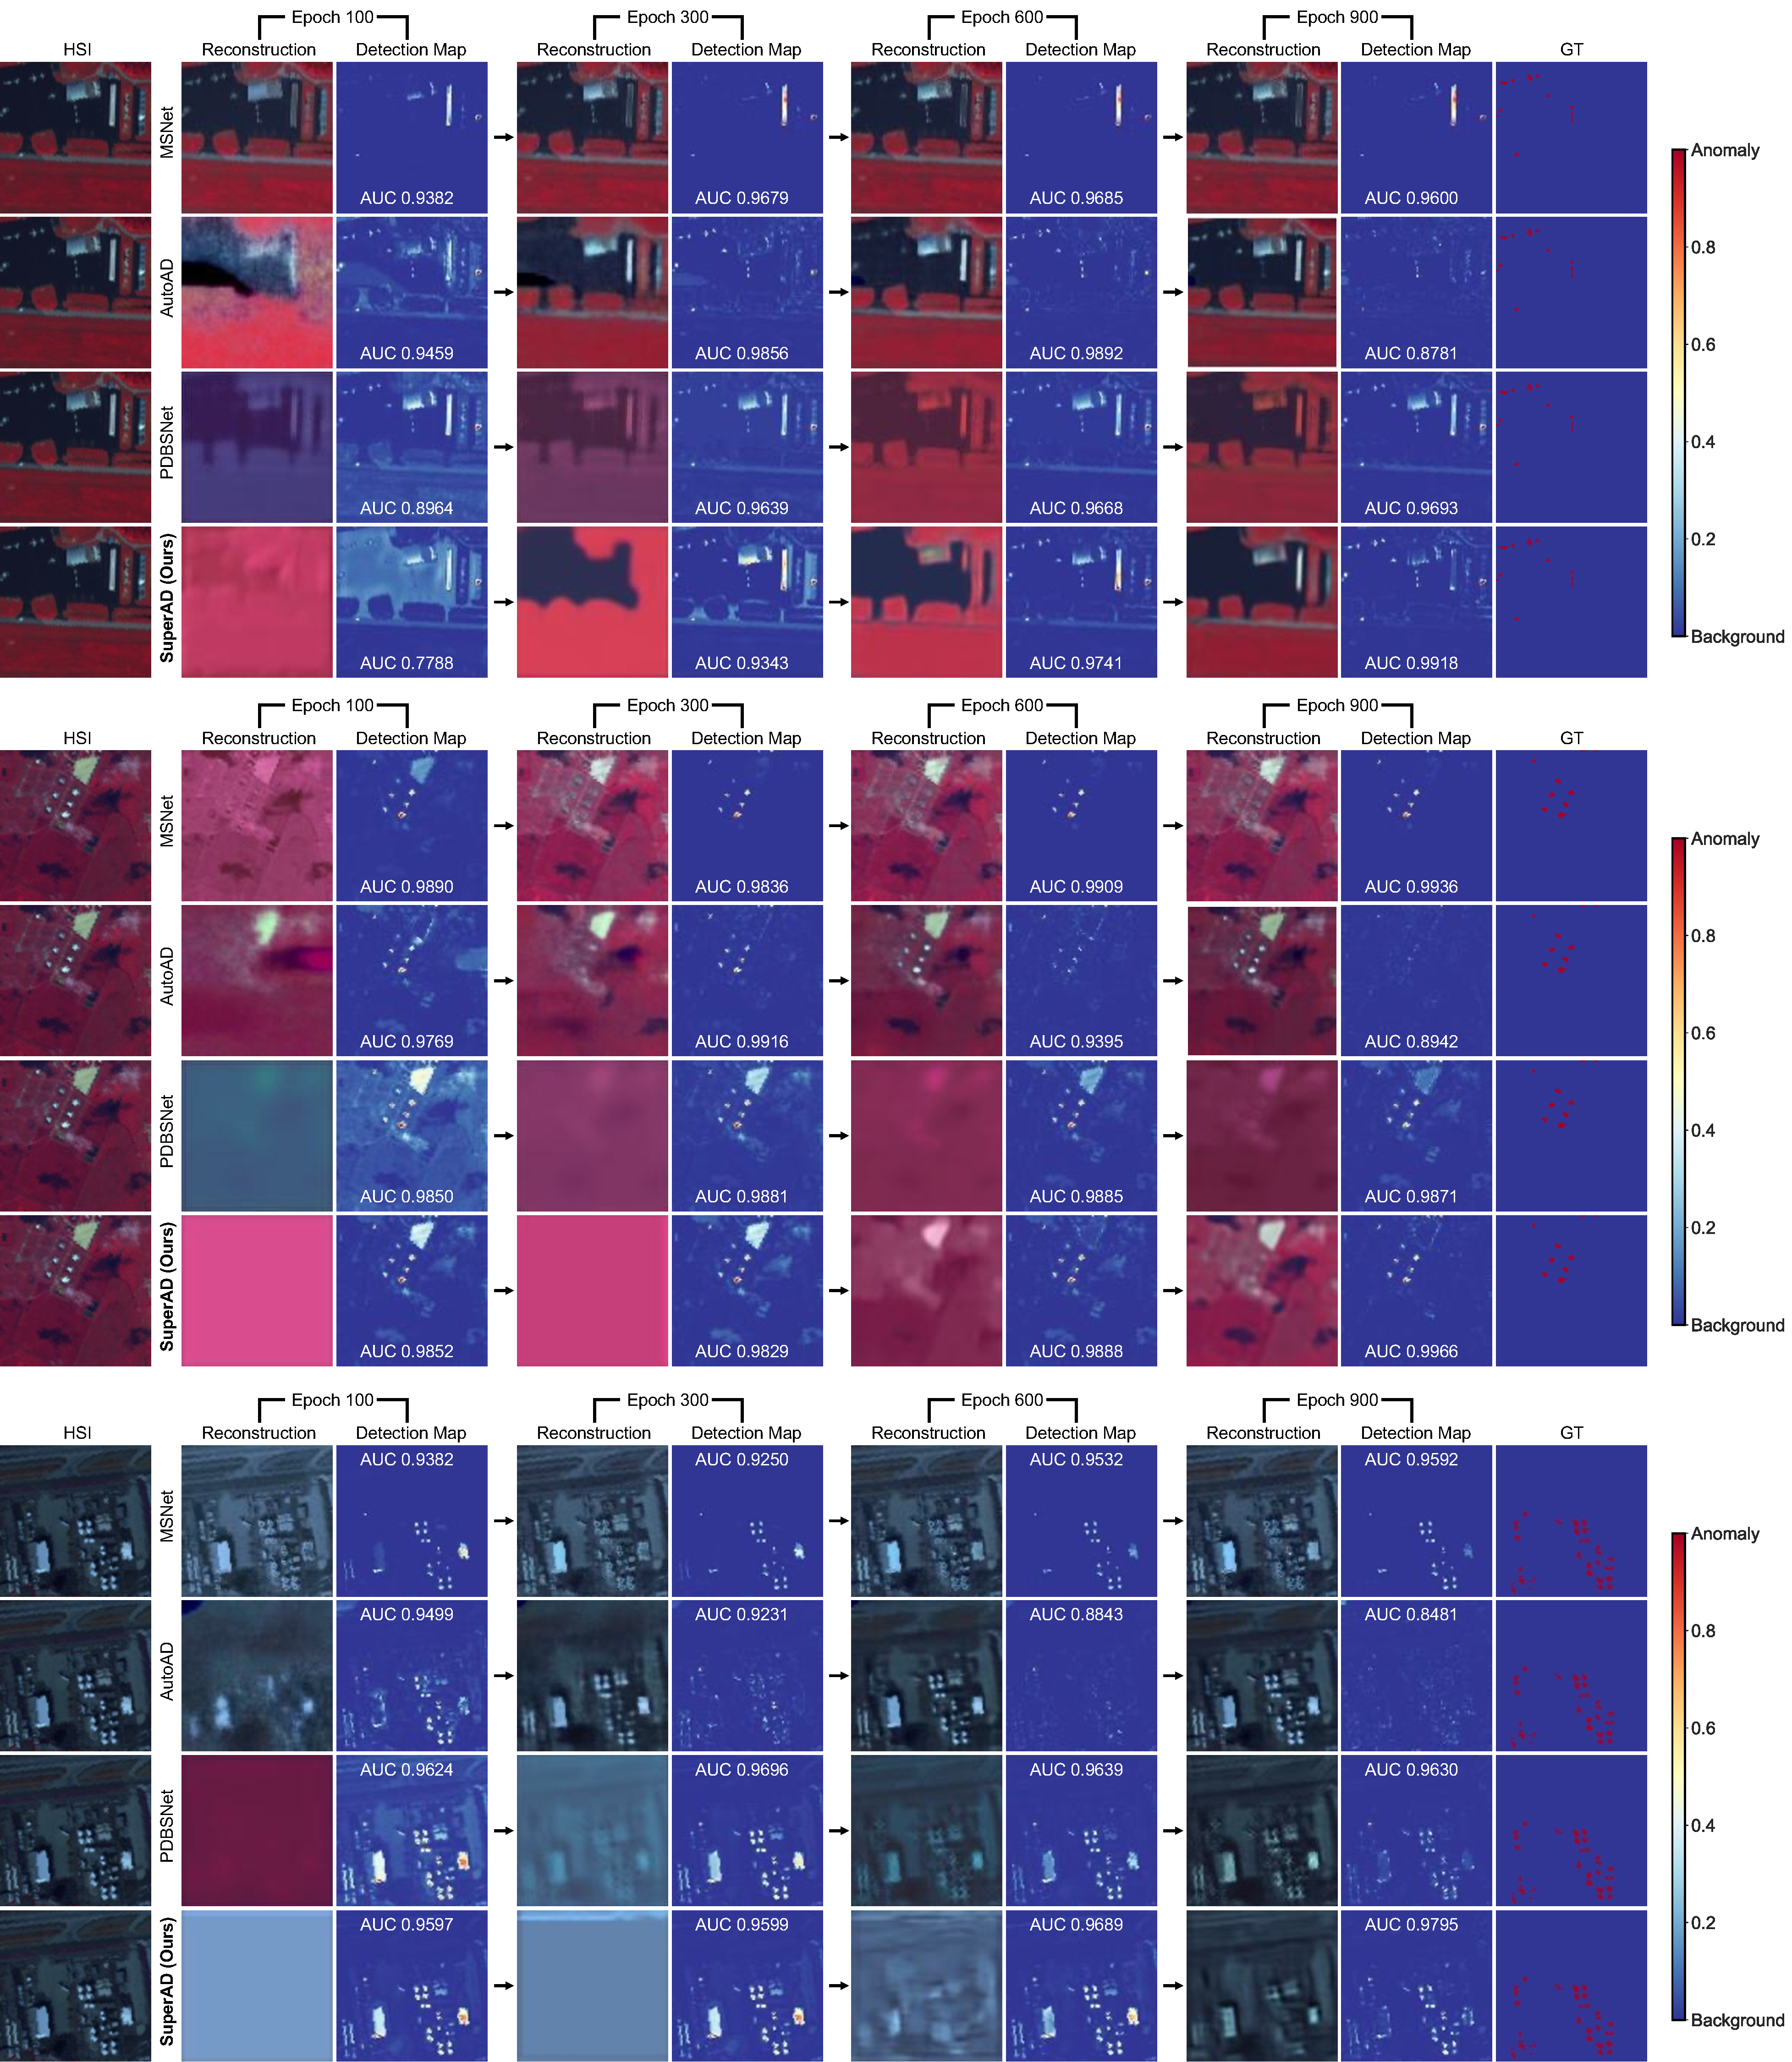
\includegraphics[width=1\linewidth]{Figures/PDF/imp_viz.pdf}
  \caption{Visualization of the reconstruction process of different detectors.}
  \label{fig:imp-viz}
\end{figure*}



\subsubsection{Regularization Term OBPM}
Fig.~\ref{fig:abl-ab} illustrates the effectiveness of the OBPM. Our method achieved an optimal AUC of $0.9961$ compared to $0.9906$ achieved by the commonly used $l_1$ or $l_2$ loss. The OBPM strategy is shown effective on reconstructing complex backgrounds while disregarding potential anomalies. The parameter sensitivity analysis reveals that the proposed OBPM performs consistently well within a range for $\beta \in [0.5, 2]$ and $\alpha \in [0, 5]$, indicating its robustness and stability across different parameter settings.



The parameter sensitivity analysis of superpixel segments, as illustrated in Fig.~\ref{fig:ana_segs}, reveals the remarkable robustness of our SPP mechanism across varying numbers of superpixel blocks. The experimental results demonstrate consistent detection performance when the number of superpixels ranges from $10$ to $900$. This stability can be attributed to the inherent property of SPP to effectively eliminate anomalous points regardless of the number of superpixel segmentation, as further validated by the detailed visualization results presented in Sec.~\ref{sec:spp} in Fig.~\ref{fig:viz-spp}. The ablation studies in Fig.~\ref{fig:ana_segs} further substantiate the essential role of both AdaConv and OBPM in our framework. The significant performance degradation observed when either component is removed underscores their critical contributions to the model's effectiveness. These findings collectively reinforce the validity and robustness of our proposed approach in addressing the IMP in self-supervised HAD.












\subsection{Visualization Analysis}


\subsubsection{Visualization of Reconstruction Results}
To better illustrate the superiority of our proposed model in addressing the IMP, we present a step-by-step visualization of the reconstruction process. We compare our model with three other reconstruction-based models (AutoAD~\cite{AutoAD}, PDBSNet~\cite{PDBSNet}, and MSNet~\cite{MSNet} ), as shown in Fig.~\ref{fig:imp-viz}. The visualization results clearly demonstrate that our model effectively mitigates the IMP throughout the training process. Specifically, as the number of epochs increases, our model consistently fails to reconstruct anomalous pixels, while successfully reconstructing the background. In contrast, AutoAD~\cite{AutoAD} tends to reconstruct the entire input image, including anomalies, leading to degraded detection performance. Similarly, PDBSNet~\cite{PDBSNet} and MSNet~\cite{MSNet} show varying degrees of anomaly reconstruction, particularly in later epochs, which compromises their ability to distinguish anomalies from the background. This comparative analysis underscores the effectiveness of our approach in preventing the reconstruction of anomalous spectra, thereby maintaining robust anomaly detection capabilities throughout the training process.


\begin{figure}[t]
  \centering
  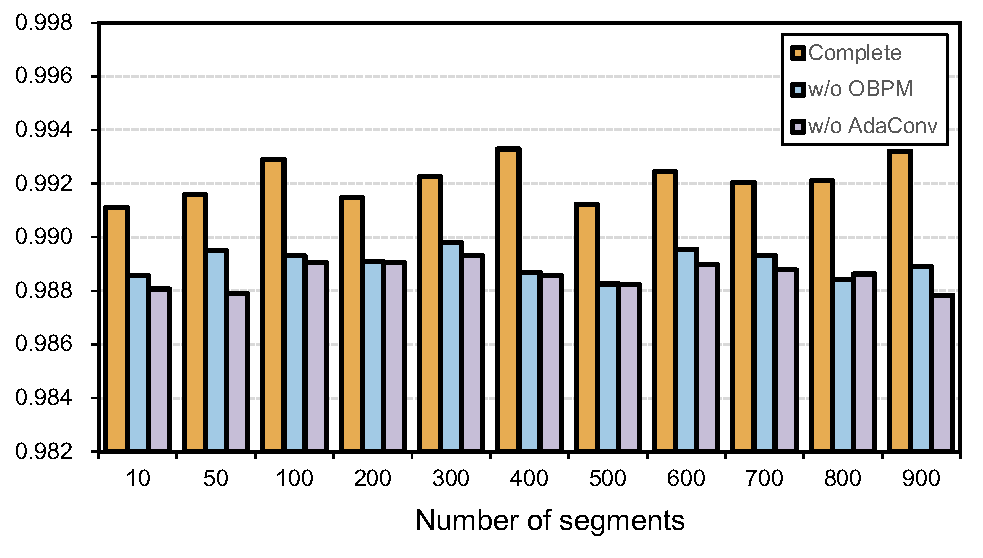
\includegraphics[width=1\linewidth]{Figures/PDF/ana_nsegs.pdf}
  \caption{Detection performance of SuperAD with different numbers of superpixel segments.}
  \label{fig:ana_segs}
\end{figure}

\begin{figure}[htbp]
  \centering
  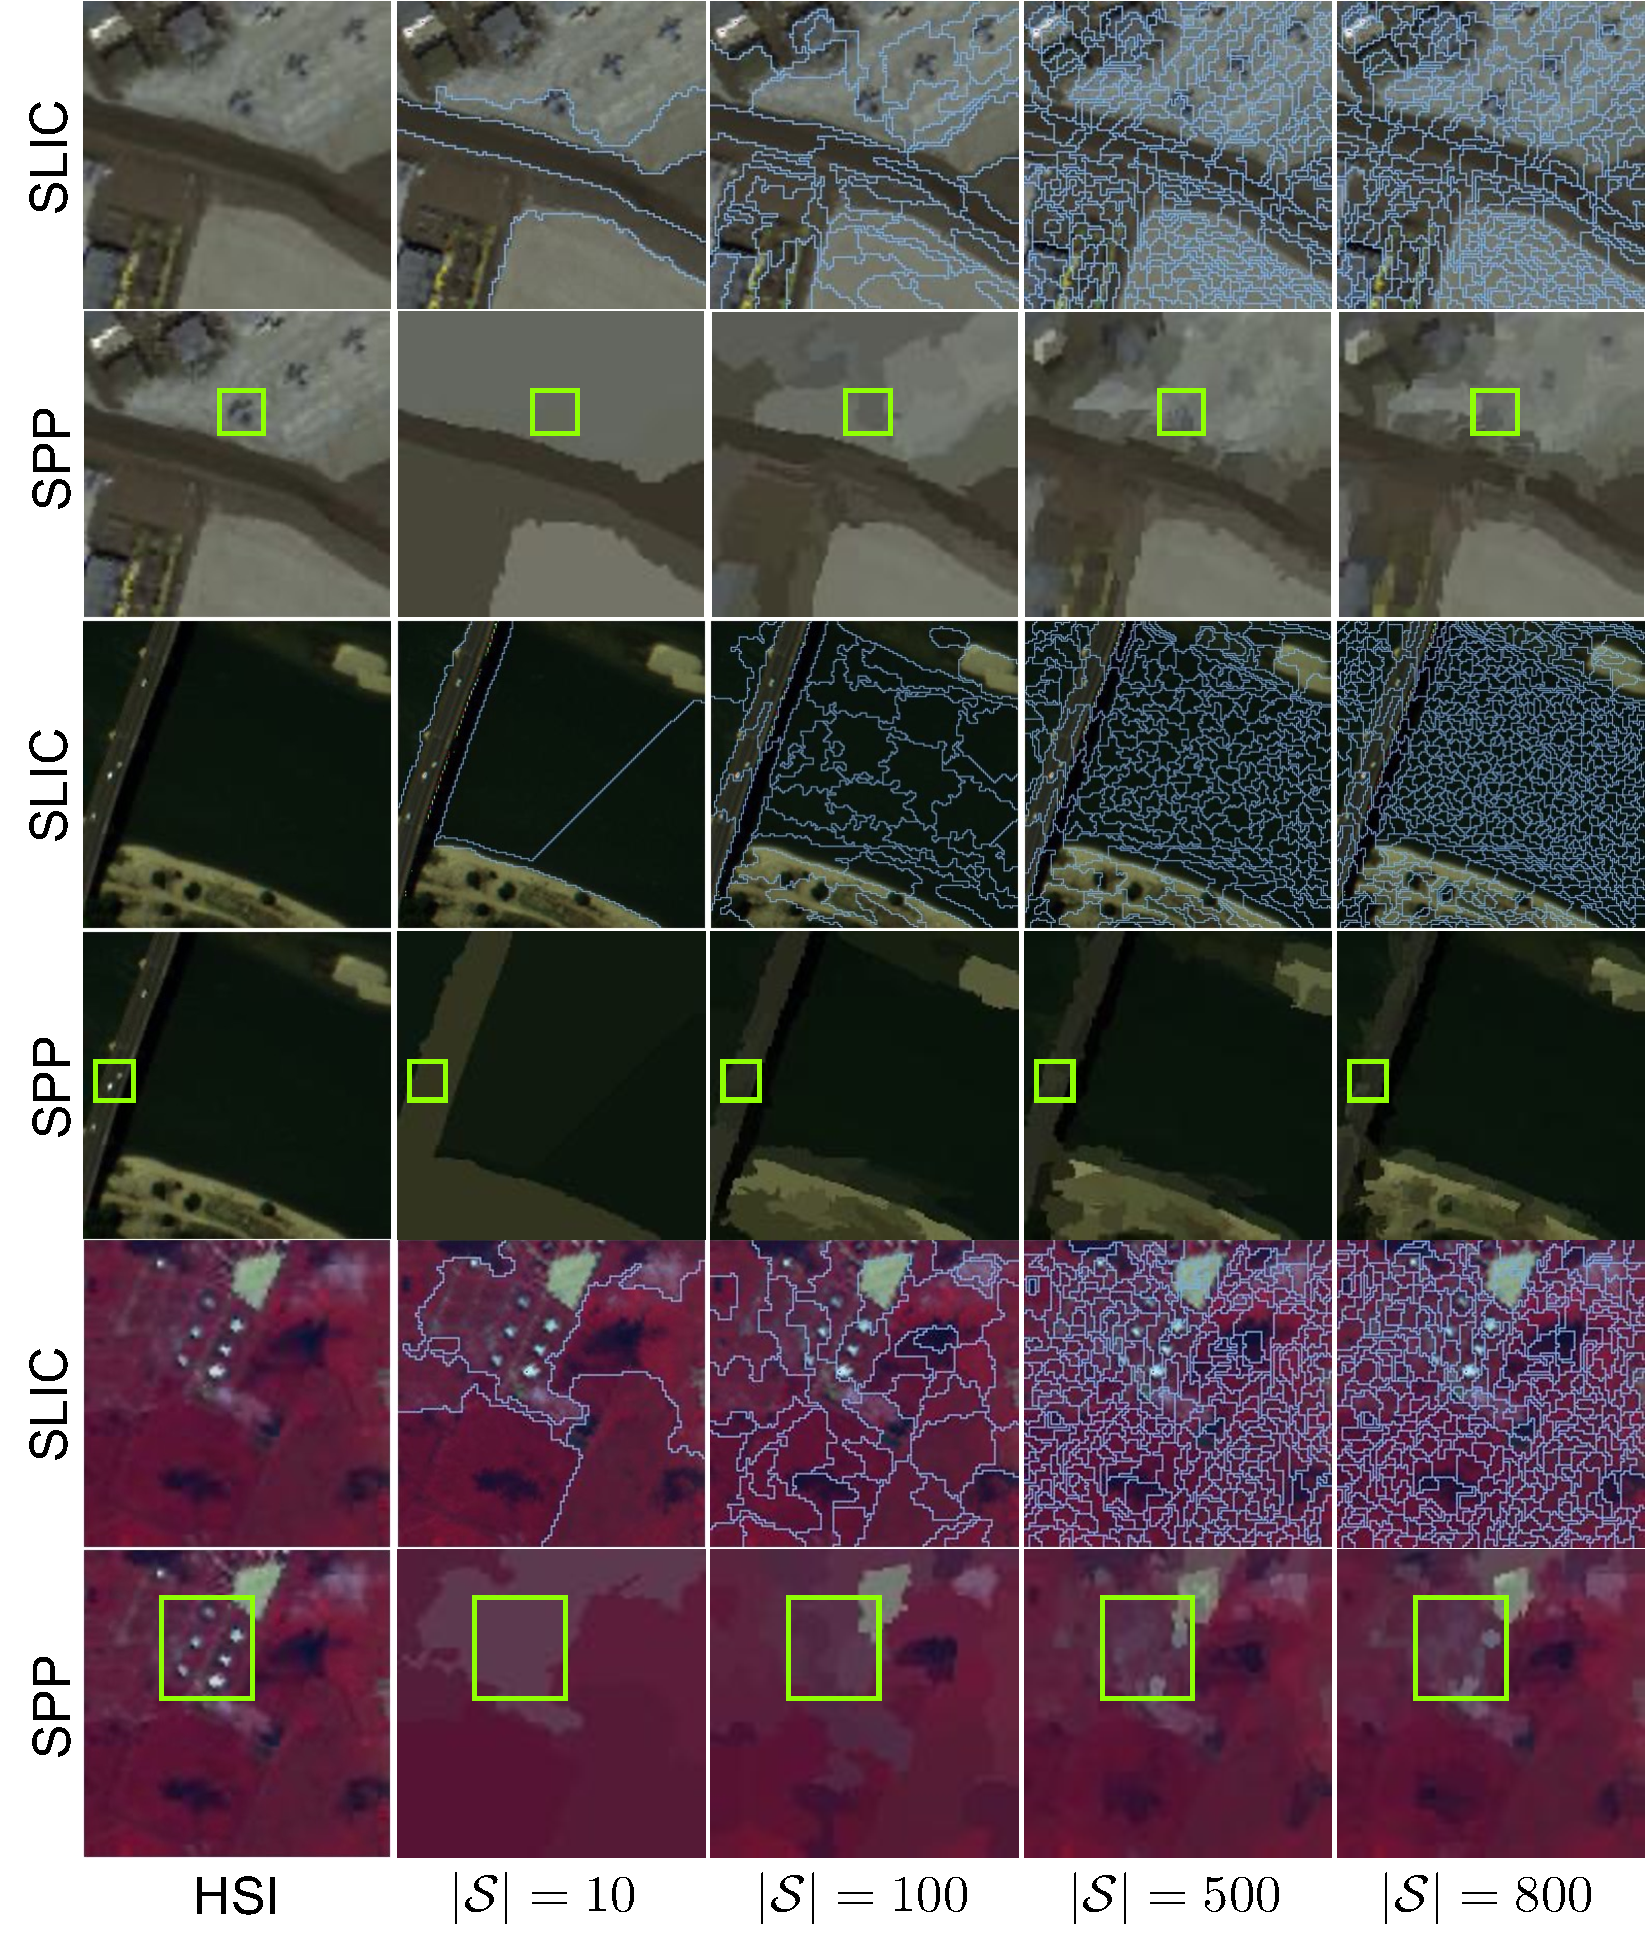
\includegraphics[width=1\linewidth]{Figures/PDF/viz_spp_slic_all.pdf}
  \caption{Visualization of superpixel pooling with different numbers of superpixels.}
  \label{fig:viz-spp}
\end{figure}



\subsubsection{Visualization of Superpixel Pooling}
Fig.~\ref{fig:viz-spp} presents a comprehensive visualization of our proposed superpixel pooling mechanism with varying numbers of superpixels, \textit{i.e.,} $|\mathcal{S}|=\{10, 100, 500, 800\}$. The highlighted regions indicate the locations of anomalous points. As the number of superpixels increases, the SPP demonstrates enhanced capability in preserving both spectral and spatial information. This is evident from the progressively detailed representation of the image structure across different superpixel counts. However, despite this increased information retention, the SPP consistently maintains its fundamental characteristic of effectively eliminating anomalous points from the reconstruction process. 

The visualization reveals that regardless of the superpixel count, the anomalous regions remain effectively suppressed in the supperpixeled images. As discussed in Sec.~\ref{sec:spp}, the stability of the SPP is also corroborated by the experimental results shown in Fig.~\ref{fig:ana_segs}, where the detection performance remains relatively stable despite variations in the number of superpixels. This parameter insensitivity is particularly advantageous in practical applications, as it reduces the need for meticulous parameter tuning while maintaining high detection accuracy. Combining the visualization results in Fig.~\ref{fig:viz-spp} and the experimental analysis in Fig.~\ref{fig:ana_segs}, our SPP approach demonstrates remarkable robustness in mitigating the influence of anomalies on the reconstruction process and thus prevents the IMP. The effectiveness of SPP can be attributed to its unique design: by encapsulating anomalous pixels within background-dominated blocks through the average pooling strategy, it inherently suppresses the influence of anomalies while preserving the essential characteristics of the background. This dual capability of information preservation and anomaly suppression contributes significantly to the overall superiority of our proposed method.



\begin{figure}[htbp]
  \centering
  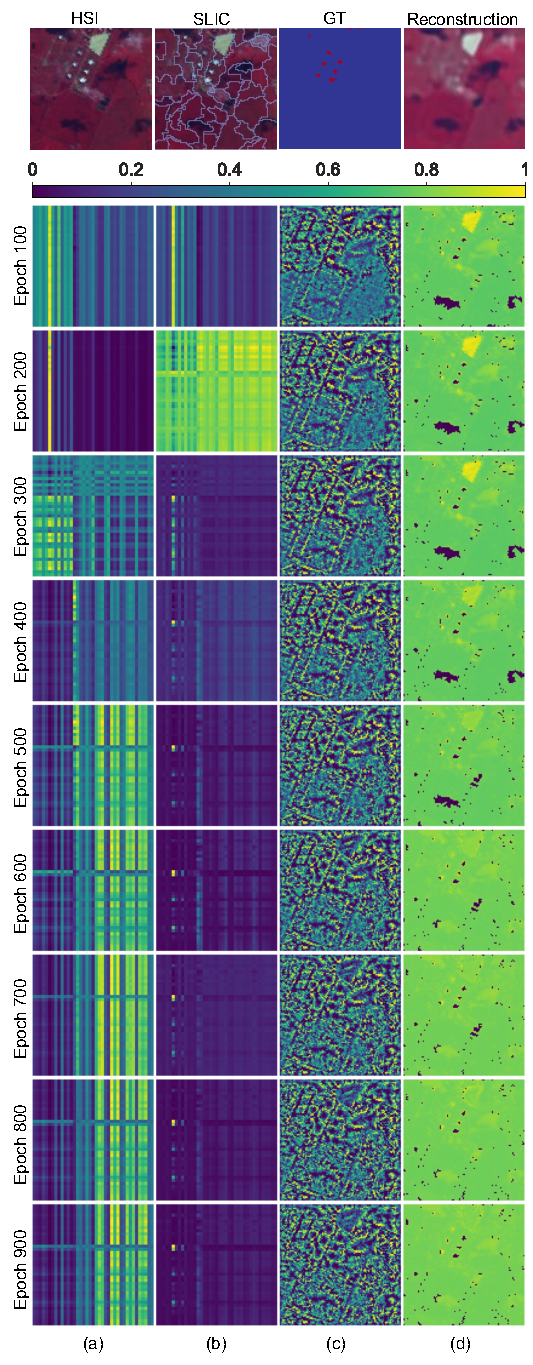
\includegraphics[width=1\linewidth]{inter_viz1.pdf}
  \caption{Visualization of training process: (a) and (b) SPP self-attention score matrices visualization. (c) AdaConv pixel utilization visualization. (d) OBPM  gradients visualization.}
  \label{fig:inter-viz}
\end{figure}


To further visualize the interaction mechanisms between different superpixel blocks during the reconstruction process, we present the attention score matrices from the first and final layers of the self-attention mechanism in SuperAD, as illustrated in Fig.~\ref{fig:inter-viz}\textcolor{blue}{(a)} and Fig.~\ref{fig:inter-viz}\textcolor{blue}{(b)}. The attention maps demonstrate that the inter-block relationships stabilize as the iteration progresses, with minimal observable changes in the attention patterns during later stages. Notably, the attention maps exhibit a vertical banded structure, indicating that the relative importance weights remain consistent for most blocks during the reconstruction process. However, a small subset of blocks, represented by the significantly brighter rows in Fig.~\ref{fig:inter-viz}\textcolor{blue}{(b)}, demonstrates unique reconstruction patterns. These blocks exhibit distinct attention distributions compared to the majority of blocks. This phenomenon suggests that while most blocks maintain consistent reconstruction dependencies, certain regions require specialized attention patterns to achieve accurate reconstruction. 


\subsubsection{Visualization of AdaConv}
Fig.~\ref{fig:inter-viz}\textcolor{blue}{(c)} presents the visualization results of AdaConv, where the kernel size and window size are configured as $3$ and $5$, respectively. The visualization is generated by accumulating the number of pixels selected by the convolution kernel during the reconstruction process, normalized to the range of $[0,1]$. A value of $0$ indicates that the corresponding pixel was never utilized throughout the reconstruction process. The visualization reveals several critical insights into AdaConv. Notably, anomalous pixels consistently demonstrate zero utilization across all epochs, indicating their complete exclusion from the reconstruction process. This selective exclusion mechanism effectively prevents the influence of anomalies on the reconstruction outcome, thereby mitigating the IMP. However, this selective process also results in the partial sacrifice of background pixel utilization. The evolution of pixel utilization patterns across different training epochs provides further insights into AdaConv. During the initial training phase (\textit{e.g.,} at epoch $100$), the utilization patterns in smooth regions of the hyperspectral image exhibit relatively similar characteristics, suggesting a more generalized approach to background reconstruction. As the training progresses to later stages (\textit{e.g.,} at epoch $900$), we observed more refined and differentiated pixel utilization patterns. As iteration gains, regions with complex spectral variations tend to exhibit higher and more diverse utilization values compared to homogeneous areas. This adaptive behavior contributes to the model's ability to accurately reconstruct intricate background patterns while maintaining its robustness against anomaly contamination. The observed characteristics of AdaConv, including its selective pixel utilization, adaptive reconstruction strategy, and progressive refinement during training, collectively contribute to its effectiveness in addressing the IMP in self-supervised HAD.



\subsubsection{Visualization of OBPM}
Fig.~\ref{fig:inter-viz}\textcolor{blue}{(d)} illustrates the visualization of the proposed online background pixel mining, where gradient values are normalized within the range of $[0,1]$. Pixels with zero values indicate spatial locations that do not contribute gradients to the backpropagation process. The visualization demonstrates a progressive learning pattern: During initial iterations, certain background regions are temporarily excluded. However, as training progresses, these background gradients are progressively reintegrated. This adaptive mechanism effectively addresses the IMP by dynamically incorporating background information while consistently filtering out anomalies. The final results show that the majority of background pixels are successfully incorporated into the model optimization, with only a minimal fraction being erroneously excluded as potential anomalies. Notably, anomalous pixels maintain zero gradients throughout the entire training process, confirming the effectiveness of OBPM in preventing anomaly reconstruction. These findings highlight OBPM's capability that dynamically adjusts background gradient utilization while strictly maintaining anomaly exclusion, thereby significantly enhancing the discriminative ability of SuperAD to distinguish normal and anomalous pixels.






























